\documentclass{article}
\usepackage{graphicx}
\usepackage[margin=1.5cm]{geometry}
\usepackage{amsmath}

\begin{document}

\title{Wednesday Reading Assessment: Unit 3, Magnetic Forces and Fields}
\author{Prof. Jordan C. Hanson}

\maketitle

\section{Memory Bank}

\begin{itemize}
\item $\vec{F} = q\vec{v} \times \vec{B}$ ... The Lorentz force
\item $\vec{x}(t) = v_{||}t \hat{i}$ ... The x-position.
\item $\vec{y}(t) = (v_{\perp}/\omega_B) \cos(\omega_B t)\hat{j}$ ... The y-position.
\item $\vec{z}(t) = (v_{\perp}/\omega_B) \sin(\omega_B t)\hat{k}$ ... The z-position.
\item $\omega_B = (q B)/m$ ... The \textit{cyclotron} frequency.
\item $\omega = 2 \pi f = 2\pi /T$ ... Relationship between angular frequency, frequency, and period.
\end{itemize}

\section{Motion of a Charged Particle in a Uniform Magnetic Field}

\begin{enumerate}
\item Consider Fig. \ref{fig:lorentz}, in which a charged particle is spiralling around a B-field. In the online video tutorial we showed that the 3D motion follows the equations in the memory bank.  (a) Where is the particle at time $t=0$?
\begin{figure}[ht]
\centering
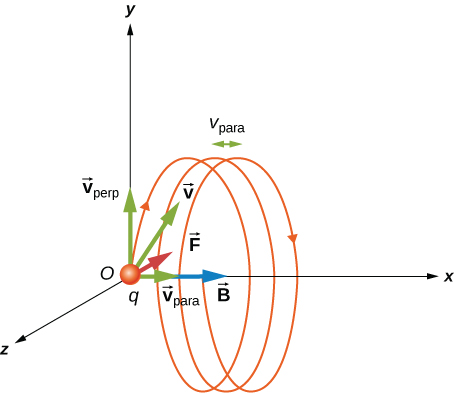
\includegraphics[width=0.25\textwidth]{lorentzSpiral.jpeg}
\caption{\label{fig:lorentz} A graph of charge passing through a certain circuit versus time.}
\end{figure}
\item If the particle starts at $(0,v_{\perp}/\omega_B,0)$, and returns there, which of the following is true of $v_{||}$?
\begin{itemize}
\item A: $v_{||} < 0$
\item B: $v_{||} > 0$
\item C: $v_{||} = 0$
\item D: $v_{||}$ is undefined.
\end{itemize}
\item Suppose the cyclotron frequency is $\omega_B = 40$ MHz, and $v_{\perp} = 10^{6}$ m/s.  What is the period of the motion around the circle? \\ \vspace{2cm}
\item What would have happened to the motion if $q < 0$?  That is, if we switch the sign of the charge, what happens to the spiral?
\end{enumerate}

\end{document}
